\chapter{HiSPARC Station 14008}\label{chap:HiSPARC_14008}

%%%%%%%%%%%%%%%%%%%%%%%%%%%%%%%%%%%%%%%%%%%%%%%%%%%%%%%%%%%%%%%%%%%%%
%%%%%%%%%%%%%%%%%%%%%%%%%%%%%%%%%%%%%%%%%%%%%%%%%%%%%%%%%%%%%%%%%%%%%
\section{Introduction}\label{sec:HS_14008_intro}

It was clear from the work covered in Chapter~\ref{chap:HiSPARC}, using data from the HiSPARC network, that the HiSPARC detectors were not clearly capable of observing space weather events and this is also hindered as they are rather sensitive to variations in the terrestrial conditions. 

To some extent, it was possible to eliminate the variation in CRs due to terrestrial variation from the HiSPARC data; however it was shown to be not always so simple, as different detectors in the HiSPARC network showed different responses to pressure and temperature variation. The non-linear relationship between temperature and CR count means the correction of the count rate due to thermal fluctuations is non-trivial, unlike the counterpart correction for pressure. 

It is believed that the atmospheric thermal fluctuations induce thermal noise in the \glspl{pmt}, and although the temperature inside the HiSPARC ski-boxes have not been measured, it is suspected that the \glspl{pmt} can get quite hot, in particular when the sky boxes are in direct sunlight.

An instance of thermal noise in a single \gls{pmt} will be random, and uncorrelated with an instance of thermal noise in another \gls{pmt}. It is therefore possible to hypothesise that it is unlikely that within the coincidence window of $\sim$1.5 $\mu \mathrm{s}$, that a coincidence between 2 \glspl{pmt} would be due to random thermal noise induced in the \glspl{pmt}.

To exploit this, it is possible to stack 2 detectors on top of each other to measure a single muon which traverses both scintillators, hence inducing signals in both \glspl{pmt}.



%%%%%%%%%%%%%%%%%%%%%%%%%%%%%%%%%%%%%%%%%%%%%%%%%%%%%%%%%%%%%%%%%%%%%
%%%%%%%%%%%%%%%%%%%%%%%%%%%%%%%%%%%%%%%%%%%%%%%%%%%%%%%%%%%%%%%%%%%%%
\section{Aims}\label{sec:HS_14008_aims}

The aim of creating a new HiSPARC station was to test whether an alternative configuration of HiSPARC station could minimise atmospheric deviations in the data and allow for the observation of space weather events...



%%%%%%%%%%%%%%%%%%%%%%%%%%%%%%%%%%%%%%%%%%%%%%%%%%%%%%%%%%%%%%%%%%%%%
%%%%%%%%%%%%%%%%%%%%%%%%%%%%%%%%%%%%%%%%%%%%%%%%%%%%%%%%%%%%%%%%%%%%%
\section{HiSPARC 14008 Detector Set-up}\label{sec:HiSPARC_14008}


%%%%%%%%%%%%%%%%%%%%%%%%%%%%%%%%%%%%%%%%%%%%%%%%%%%%%%%%%%%%%%%%%%%%%
\subsection{Configuration}

The configuration of HiSPARC station 14008 is shown in Figure \ref{fig:14008_config}; the station is composed of two scintillators stacked on top of each other, inside one ski-box. 

Each of the plastic scintillators has a thickness of $\Delta x \, = \, 0.5$~cm, and density, $\rho \, = \, TBC$~gcm$^{-3}$ . We know that the stopping power of the scintillator for a minimum ionising particle is $\sim 2$~MeV/cm$^{-2}$ [REF]... [discuss this w/ Angela as it seems to be derivative of Blethe-Bloch, but cannot find link]...

\begin{figure}
	\center
	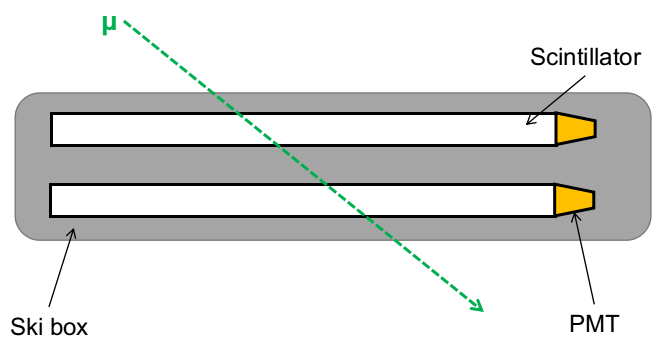
\includegraphics[width=0.5\columnwidth]{14008_config.png}
	\caption{Schematic diagram of the HiSPARC station 14008 detector set-up.}
	\label{fig:14008_config}
\end{figure}

\begin{equation}
E = \Delta x \, S \, \rho \, \cos(\theta)
\label{eq:energy_loss}
\end{equation}

\cite{bartels_hisparc_2012} state that typical energy loss of a muon in a single scintillator is $3.38$~MeV, hence in this configuration, as a muon traverses two scintillators, the lower limit on the energy loss by muons in the detector is $\sim 6.76$~MeV.

To protect the scintillators and \glspl{pmt} within the ski boxes, we sandwiched the scintillators between layers of foam, as can be seen on the lab work bench in Figure~\ref{fig:14008_detectors}. Upon complete assembly of the detector, the scintillators and \glspl{pmt} are placed within the ski-box on the roof of the Poynting Physics building on the campus of the University of Birmingham, as shown in Figure~\ref{fig:14008_ski_box}.

\begin{figure}[ht]
	\centering
	\subfloat[Scintillators on the work bench]{
		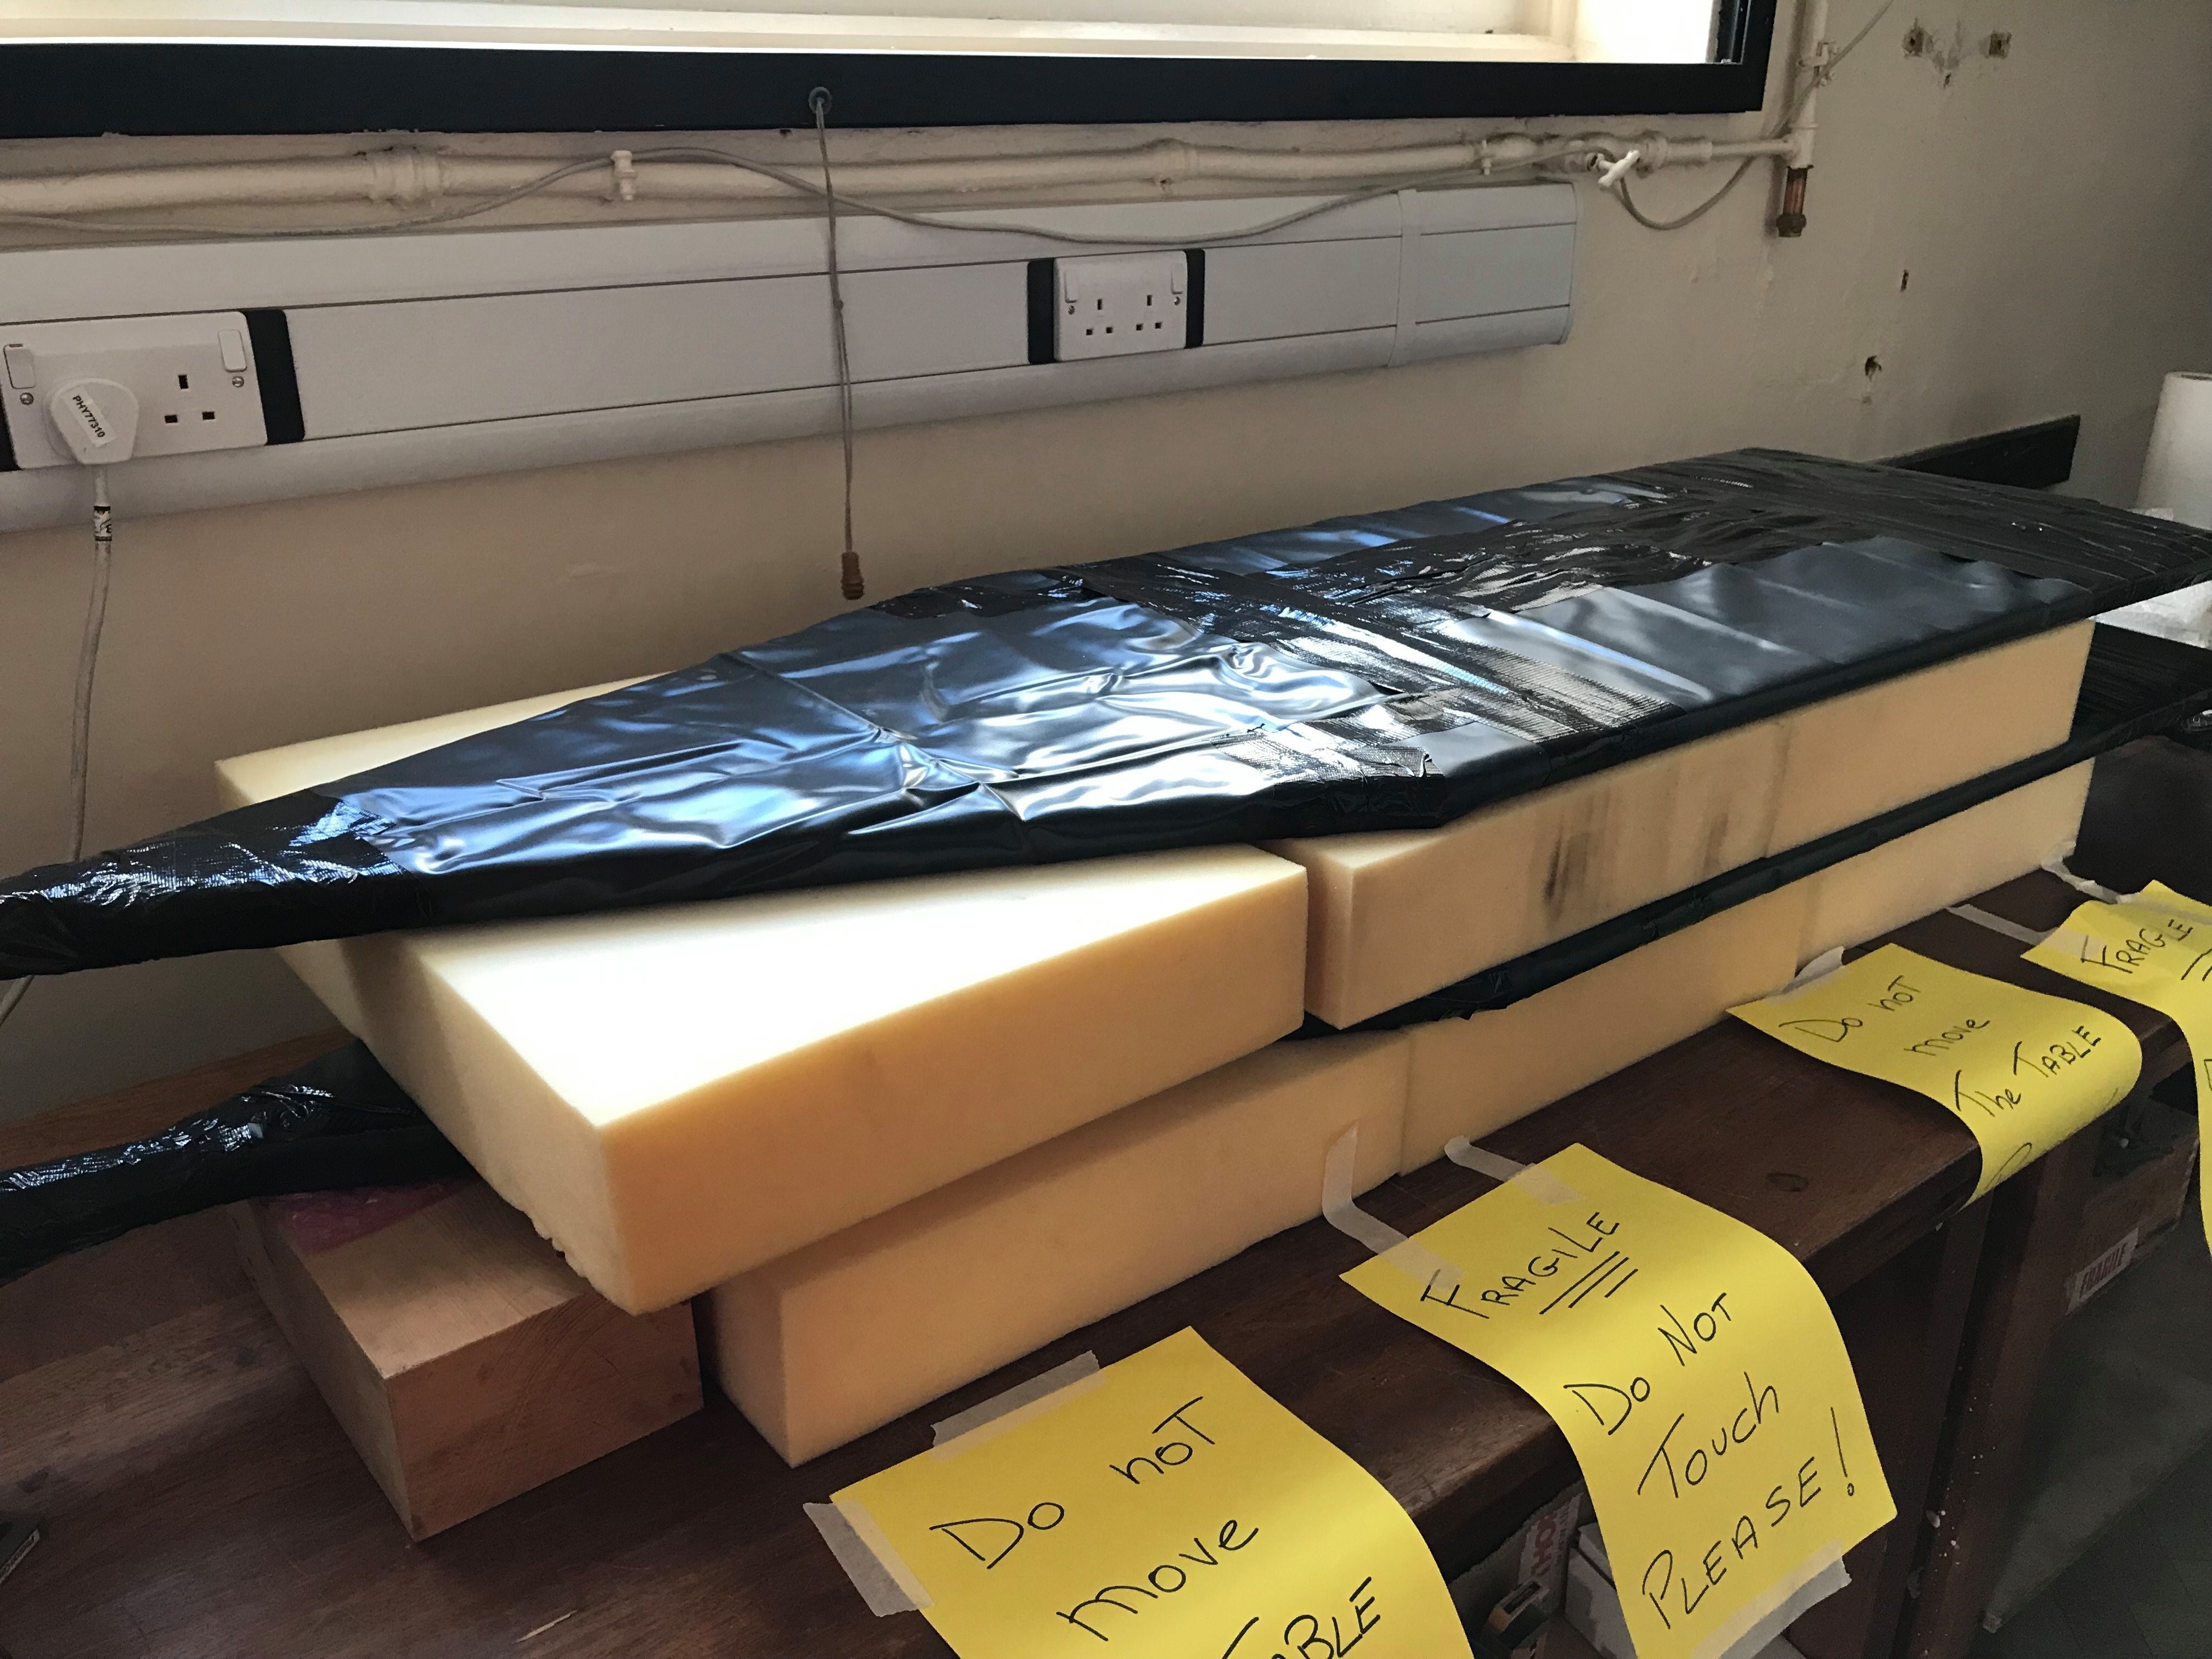
\includegraphics[width=0.48\columnwidth]{detectors.jpg}
		\label{fig:14008_detectors}}
	%\qquad
	\subfloat[Complete detector on the roof]{
		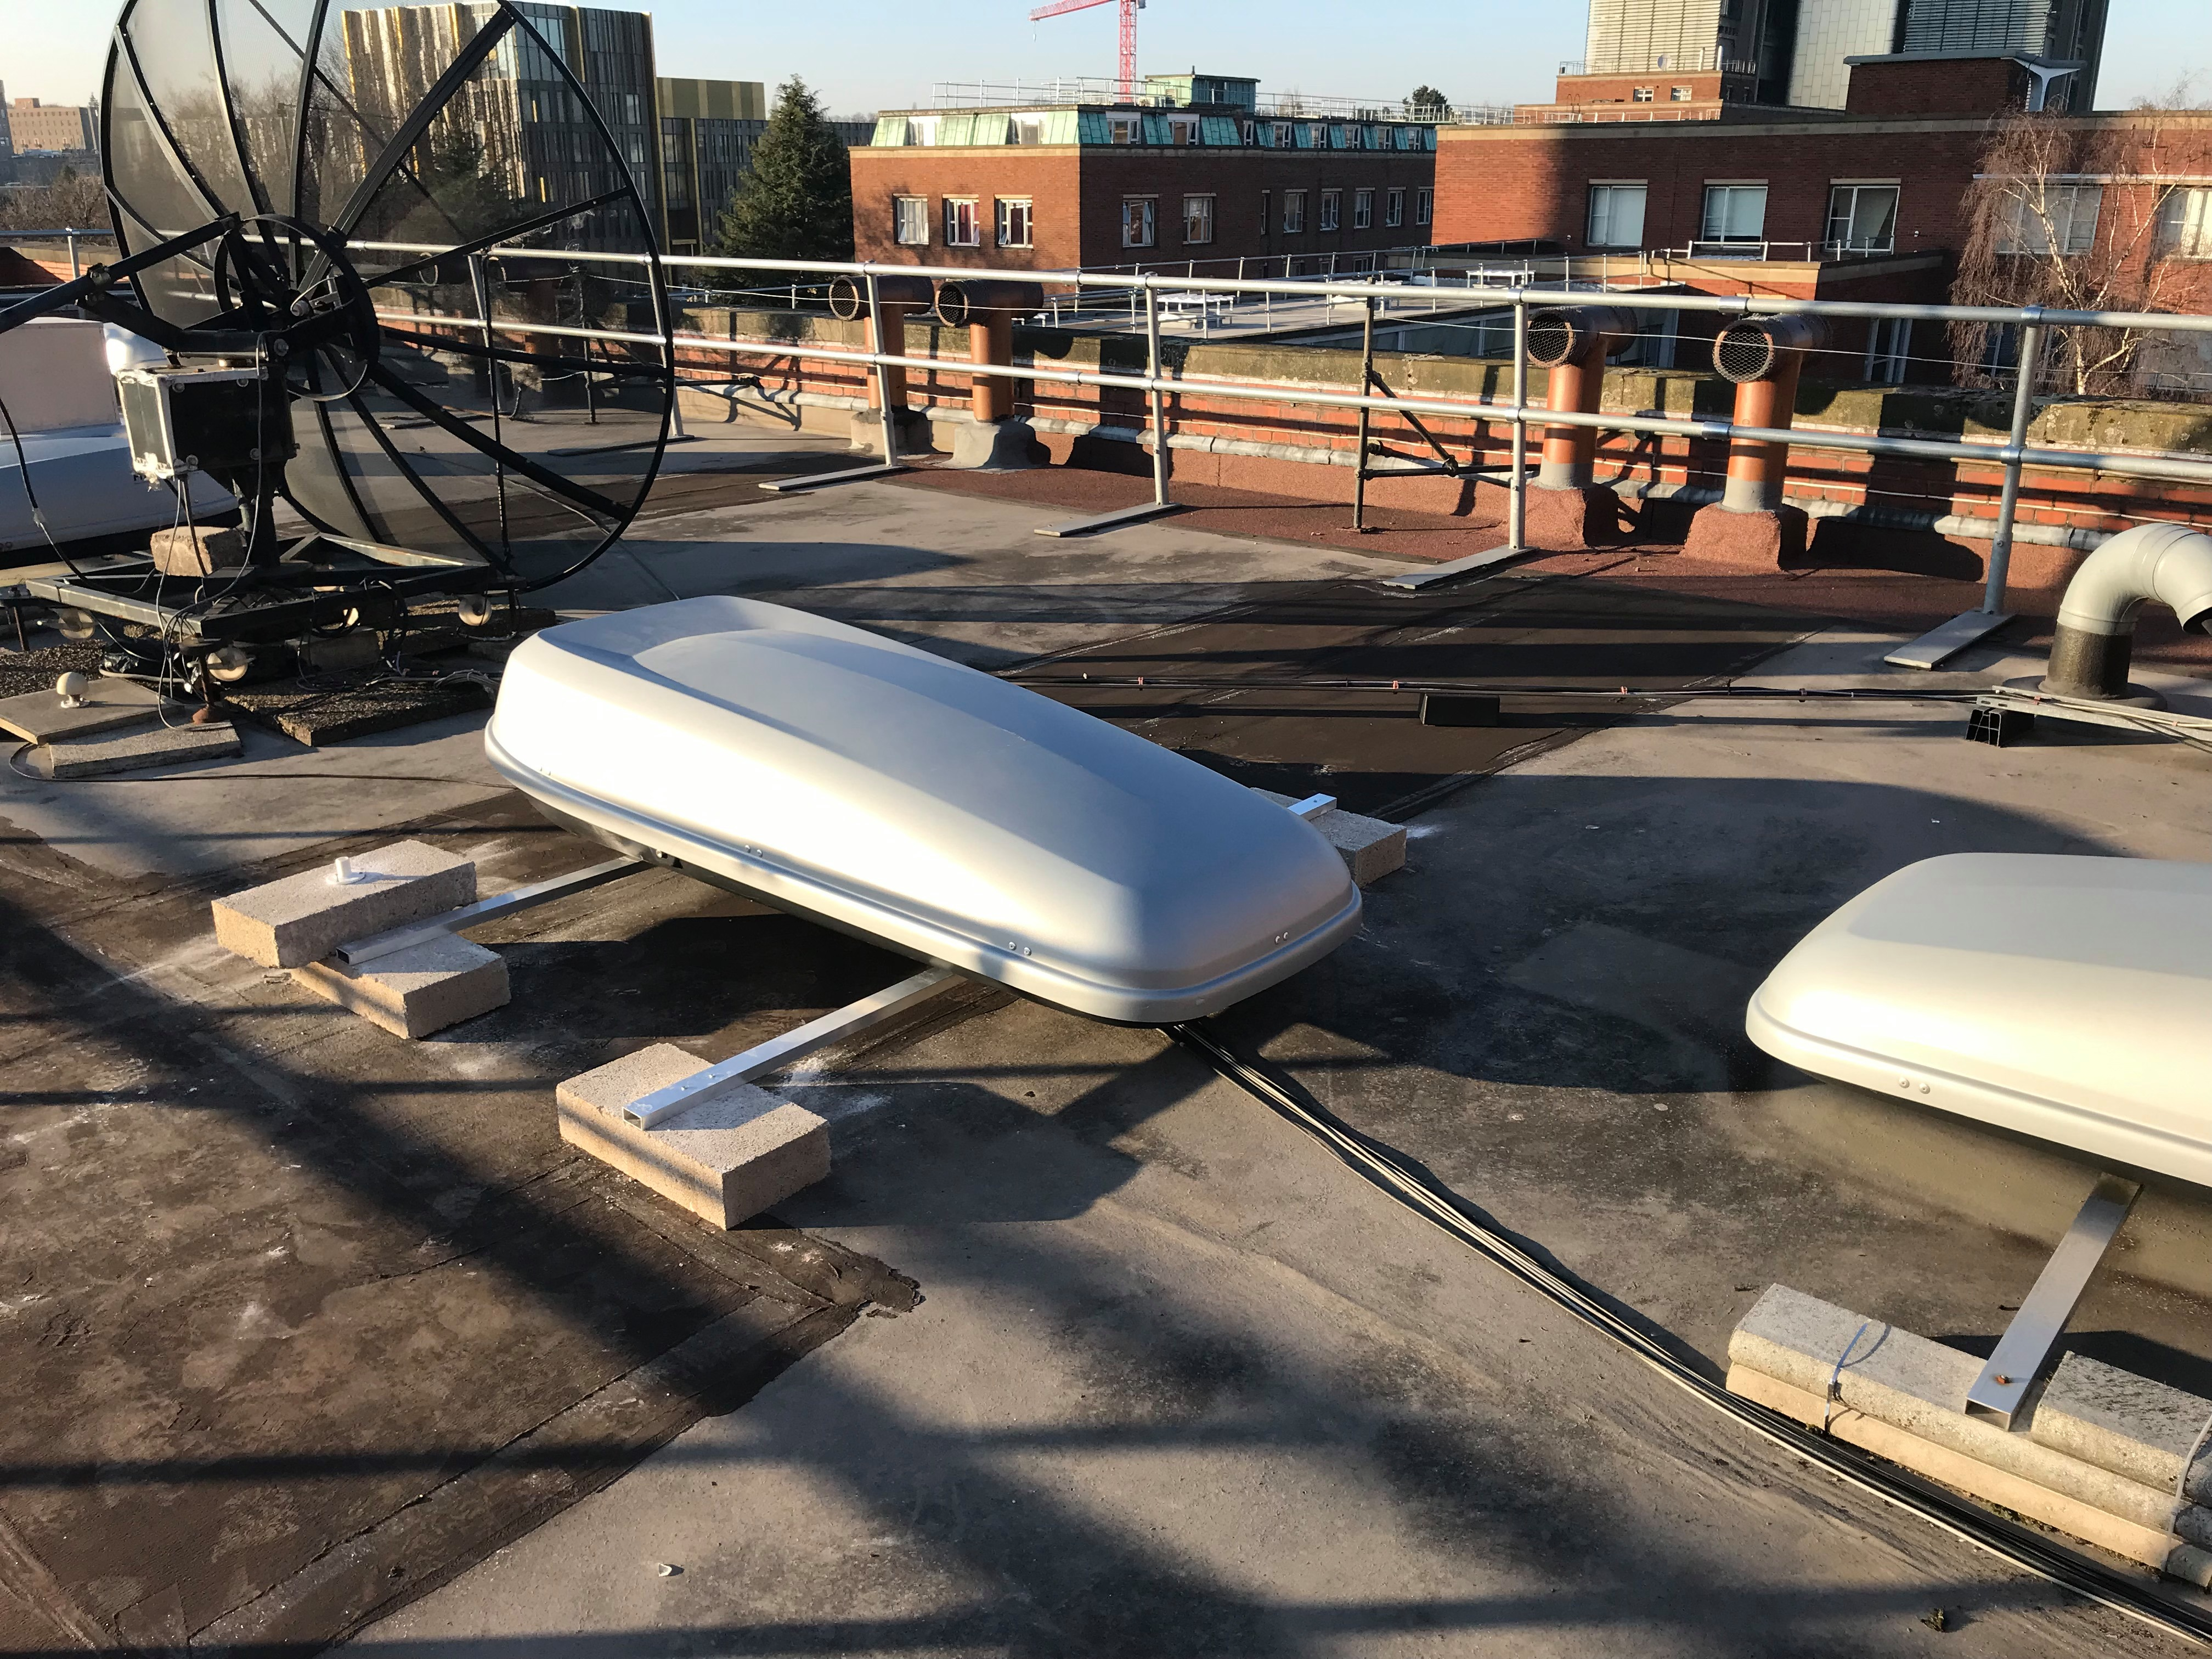
\includegraphics[width=0.48\columnwidth]{ski_box.jpg}
		\label{fig:14008_ski_box}} \\
	
	\caption{HiSPARC 14008 assembly and configuration. (a) shows the stacked arrangement of the scintillators on the lab work bench, between layers of pretective foam. (b) shows the complete detector inside the ski-box on the University of Birmingham campus.}
	\label{fig:HS_14008_setup}
\end{figure}


%%%%%%%%%%%%%%%%%%%%%%%%%%%%%%%%%%%%%%%%%%%%%%%%%%%%%%%%%%%%%%%%%%%%%
\subsection{Calibration}

When setting up the HiSPARC station, it was required to set several operating parameters for the detectors and the HiSPARC electronics box. One such setting was the \gls{pmt} operating voltage. Each of the detector \glspl{pmt} needs to be powered with a high enough operating voltage such to provide an amplified signal, but not too high such as to over-amplify the noise.

In general, the \glspl{pmt} has an advised operating voltage of around 700~V \citep{fokkema_hisparc_2019}; however, best practise is to operate the \gls{pmt} at the plateu region, whereby the counts/voltage no longer increases. As can be seen from Figure~\ref{fig:PMT_cal}, neither of the \glspl{pmt} have clear plateau regions, hence there was no obvious \gls{pmt} set point.

The HiSPARC installation manual does, however, suggest to tune the \gls{pmt} voltages such that the singles rates for each detector meet the following criteria: singles rate of 100--130 Hz for signal above the high trigger threshold, and singles rate of $<$400 Hz for signal above the low trigger threshold \citep{fokkema_hisparc_2019}.

In order to calibrate the \glspl{pmt} to the correct level, we measured the singles rates above the high and low thresholds as a function of \gls{pmt} operating voltage, as is shown in Figure~\ref{fig:PMT_cal} [UPDATE THIS PLOT...!!!!]. The voltage calibration plot shows drastically the different performances one can get from different \glspl{pmt}, therefore it is necessary to treat each \gls{pmt} individually when calibrating.

\begin{figure}
	\centering
	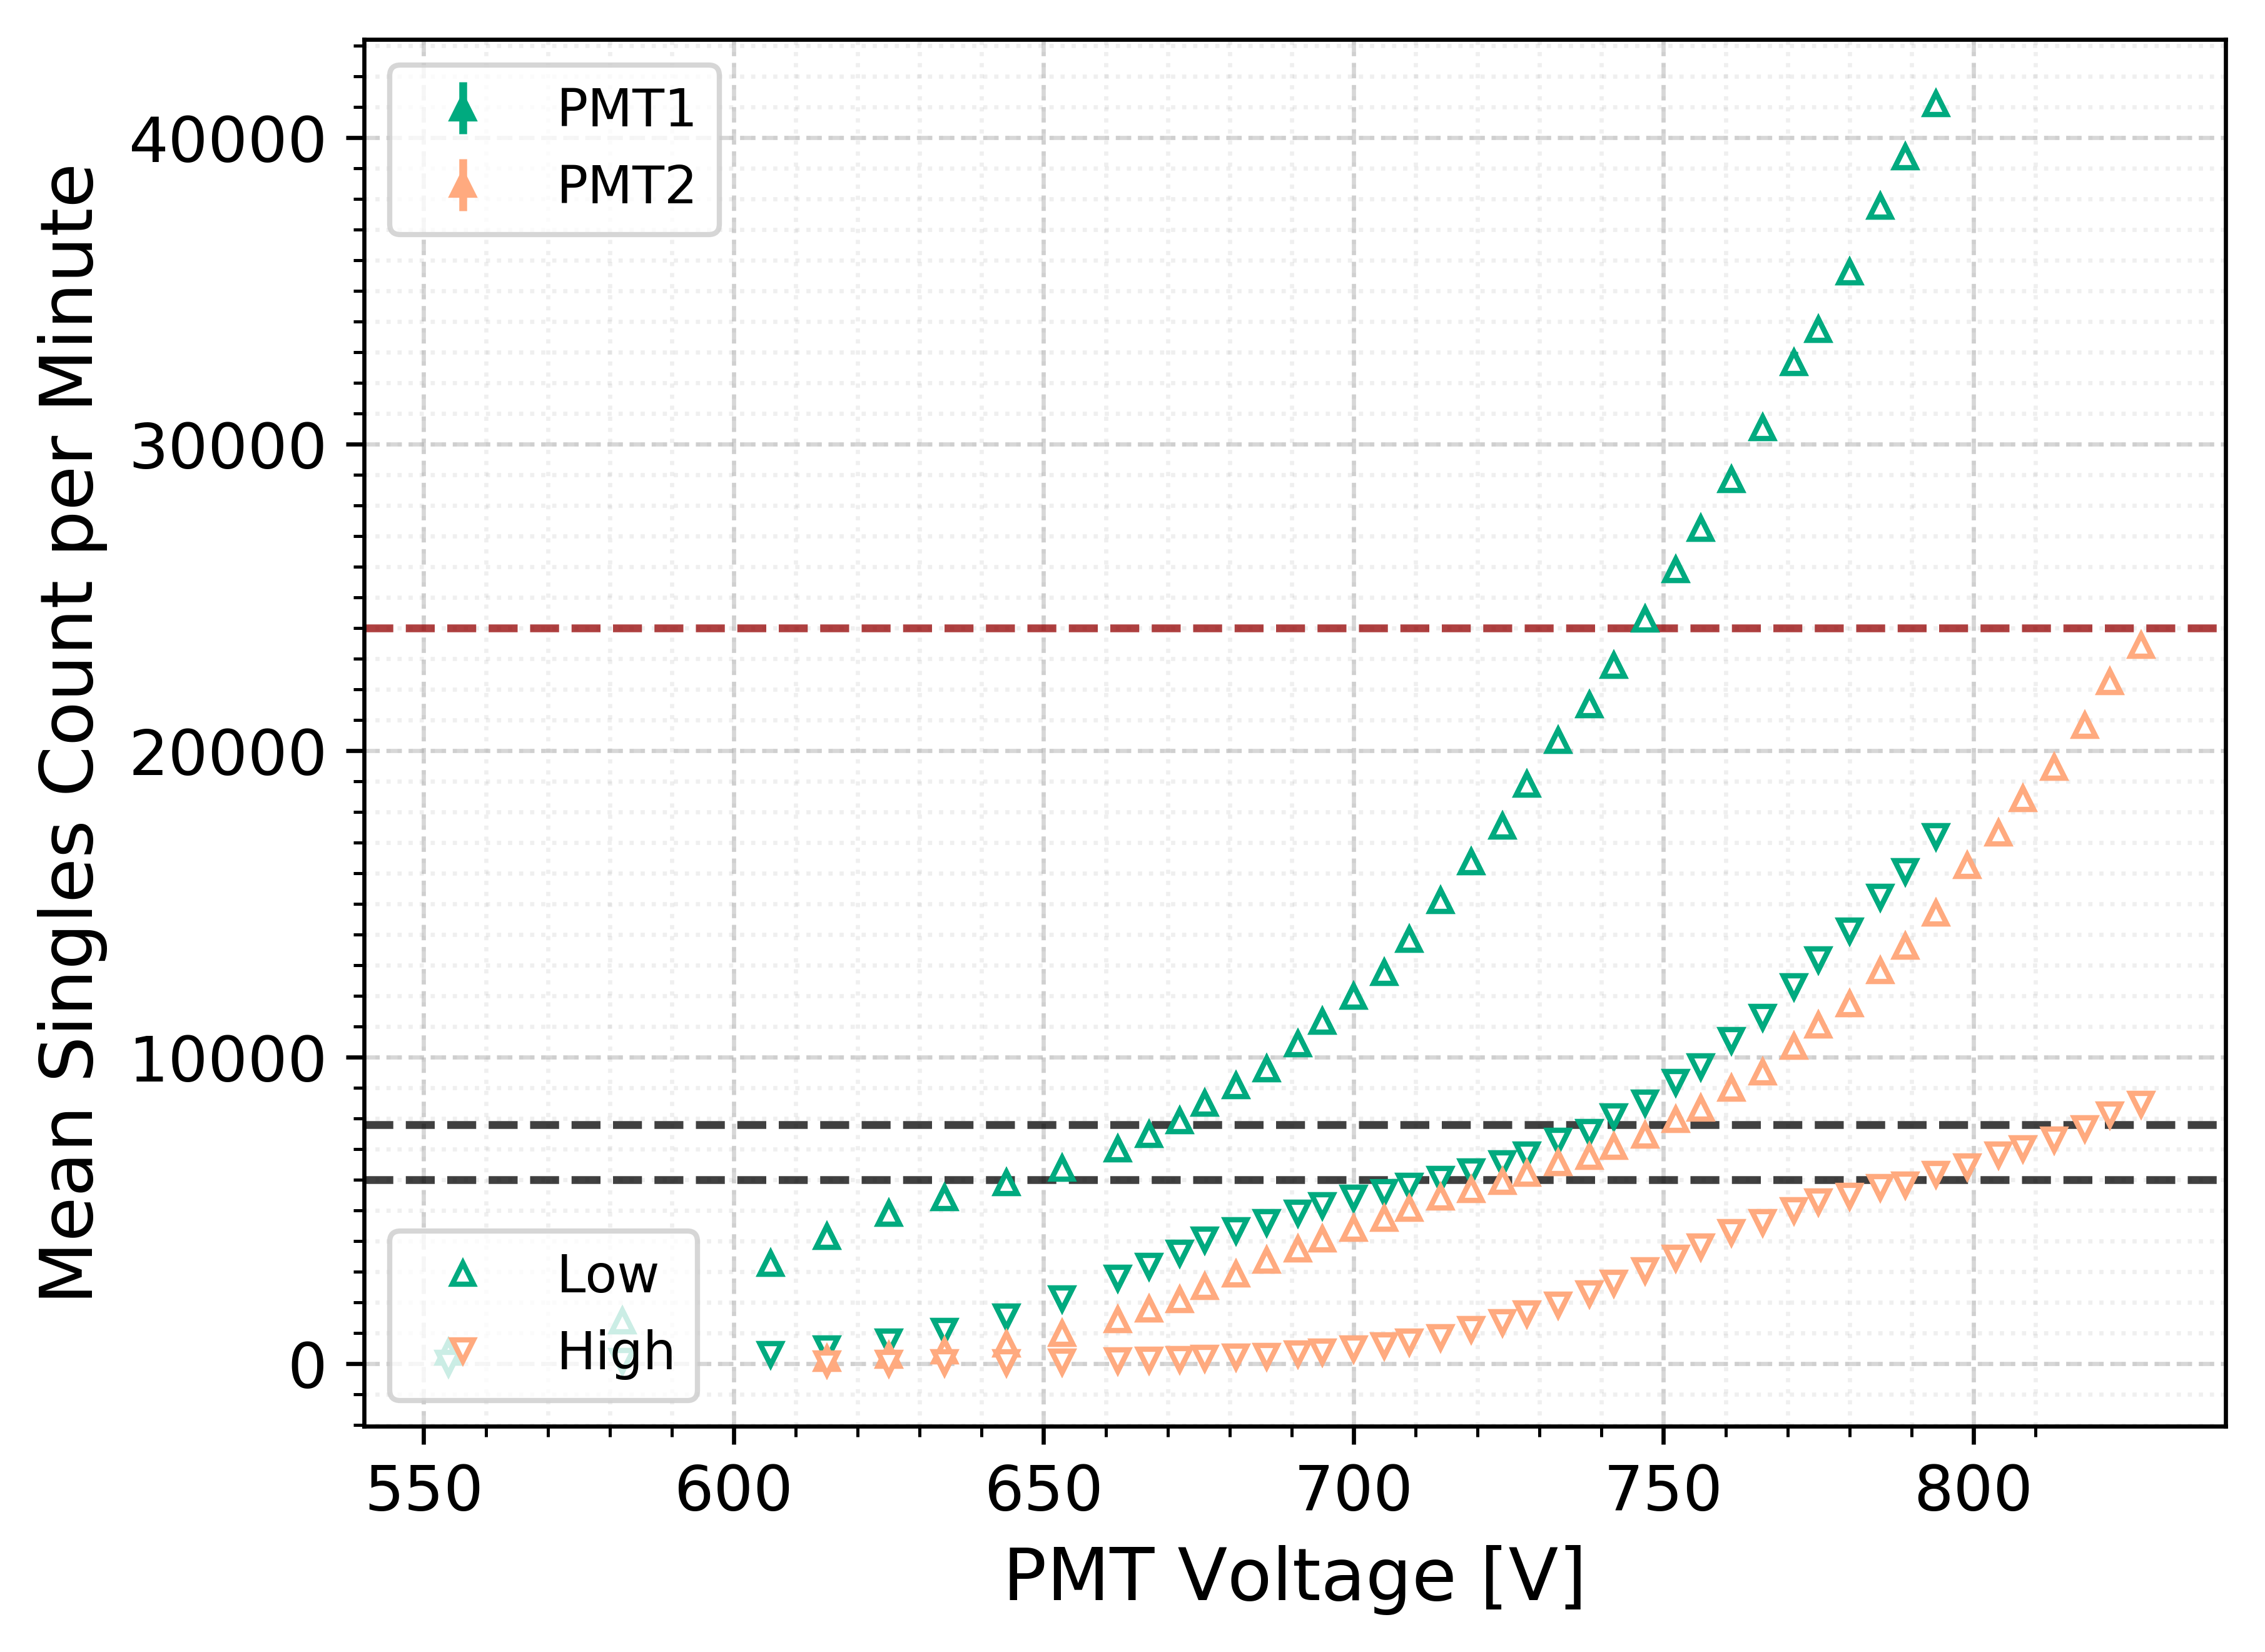
\includegraphics[width=0.75\columnwidth]{both_PMTs_post_NIM.png}
	\caption{Voltage calibration curve for the PMTs of station 14008. The upper, red-dashed line indicates the upper limit for the low threshold singles rate (400 Hz), and the lower 2, black-dashed lines indicate the upper and lower bounds for the high threshold singles rate (100--130 Hz).}
	\label{fig:PMT_cal}
\end{figure}




%%%%%%%%%%%%%%%%%%%%%%%%%%%%%%%%%%%%%%%%%%%%%%%%%%%%%%%%%%%%%%%%%%%%%
\subsection{Monitoring Temperature}

It was suspected in Chapter~\ref{chap:HiSPARC} that the singles count rates (and thus event count rates also) are affected by the temperature of the \gls{pmt} within the HiSPARC ski-boxes.

Some of the existing HiSPARC stations monitor local temperature however none measure the temperature of the \gls{pmt} within the ski box; therefore the temperature of the PMT itself is unknown, and thus we cannot account for the thermal noise. When building this new HiSPARC station, a temperature sensor was placed into the ski box which allowed us to monitor the temperature.

Figure~\ref{fig:temperature_sensor_circuit} shows the schematic for the temperature sensor. We used the DS18B20 temperature sensor with the one-wire telemetry protocol, which used a single wire to transmit the temperature readings to the microcontroller; the microcontroller used was a Raspberry Pi 4. Three wires were used for the operation of the DS18B20: constant current voltage, ground, and data.

\begin{figure}
	\centering
	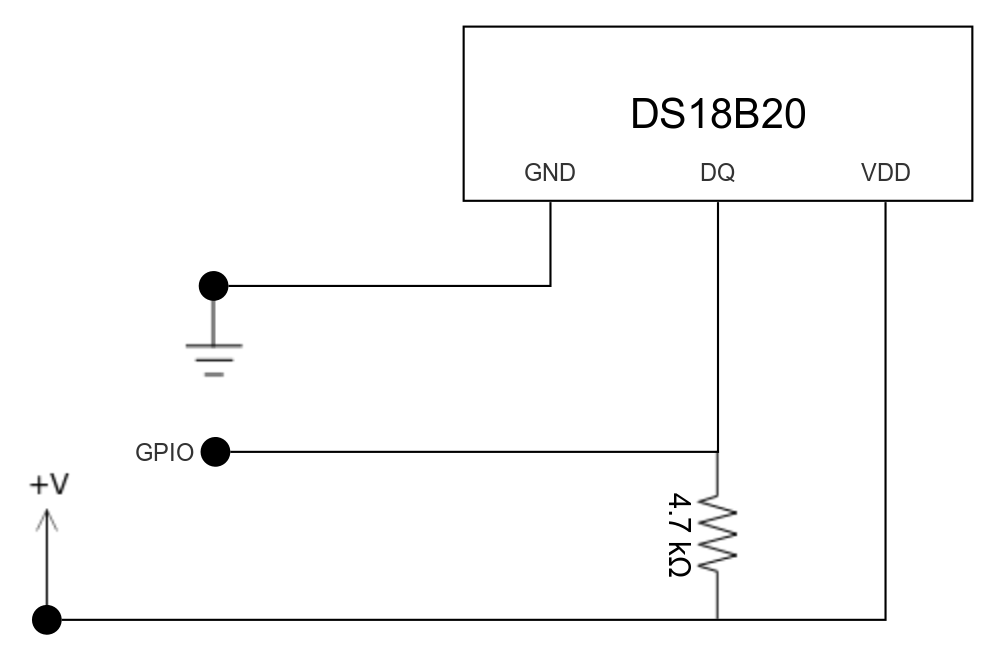
\includegraphics[width=0.6\columnwidth]{HS_14008_temp_circuit.png}
	\caption{Schematic diagram of the DS18B20 temperature sensor circuit, whereby the voltage, ground, and GPIO interfaces connect directly into pins of the Raspberry Pi board.}
	\label{fig:temperature_sensor_circuit}
\end{figure}

We use the Raspberry Pi to control the data acquisition by running a Python program to output the temperature readings from the sensor to a local file. The temperature is read on a 10-second cadence and is recorded in degrees Celsius.

%%%%%%%%%%%%%%%%%%%%%%%%%%%%%%%%%%%%%%%%%%%%%%%%%%%%%%%%%%%%%%%%%%%%%
%%%%%%%%%%%%%%%%%%%%%%%%%%%%%%%%%%%%%%%%%%%%%%%%%%%%%%%%%%%%%%%%%%%%%
\section{Observations}\label{sec:HS_14008_observations}

From the \gls{corsika} simultions in the earlier section, we predict a ground level muon rate passing through the detectors...

(do this by intergrating under curve, using 70-degre half-angle cone for solid angle, and area of 0.5m2)
% i.e. in python doing doing:
% where df contains the alpha and proton diff fluxes
% v = scipy.integrate.simps(df_a_v[1]+df_p_v[1], df_a_v.index.values)
% sr = 4*np.pi*(np.sin(np.deg2rad(70/2)))**2
% area = 0.5
% rate_v = v*sr*area

Get the rate as: $85.365 \, \mu/\mathrm{s}$ (non-vertical, i.e. 70-deg sims) or $156.924 \, \mu/\mathrm{s}$ (for vertical sims)

... for a typical day with this station, we have a count rate of $\sim 80 \, \mu/\mathrm{s}$...

%%%%%%%%%%%%%%%%%%%%%%%%%%%%%%%%%%%%%%%%%%%%%%%%%%%%%%%%%%%%%%%%%%%%%
%%%%%%%%%%%%%%%%%%%%%%%%%%%%%%%%%%%%%%%%%%%%%%%%%%%%%%%%%%%%%%%%%%%%%
\section{Conclusions}\label{sec:HS_14008_conclusion}
